\documentclass[12pt,a4paper]{article}
\usepackage[utf8]{inputenc}
\usepackage[croatian]{babel}
\usepackage{geometry}
\usepackage{graphicx}
\usepackage{pgfplots}
\pgfplotsset{compat=1.18}
\usepackage{booktabs}
\usepackage{xcolor}
\usepackage{hyperref}
\usepackage{enumitem}
\usepackage{fancyhdr}
\usepackage{listings}
\usepackage{float}

\geometry{margin=2.5cm}

% Boje za ozbiljnost
\definecolor{critical}{RGB}{220, 53, 69}
\definecolor{high}{RGB}{255, 193, 7}
\definecolor{medium}{RGB}{255, 152, 0}
\definecolor{low}{RGB}{40, 167, 69}

% Header i Footer
\pagestyle{fancy}
\fancyhf{}
\fancyhead[L]{\leftmark}
\fancyhead[R]{Izvještaj o Inspekciji Koda}
\fancyfoot[C]{\thepage}
\renewcommand{\headrulewidth}{0.4pt}
\renewcommand{\footrulewidth}{0pt}

% Hyperref postavke
\hypersetup{
    colorlinks=true,
    linkcolor=blue,
    filecolor=magenta,      
    urlcolor=cyan,
    pdftitle={Izvještaj o Inspekciji Koda - RestaurantInventory},
    pdfauthor={Tim 4}
}

\title{\textbf{Izvještaj o Inspekciji Koda}\\
\large RestaurantInventory - Tim 4}
\author{}
\date{}

\begin{document}

\maketitle
\thispagestyle{empty}

\vspace{2cm}

\begin{center}
\textbf{Informacije o Inspekciji}
\end{center}

\begin{table}[H]
\centering
\begin{tabular}{ll}
\textbf{Datum inspekcije:} & \today \\
\textbf{Moderator inspekcije:} & Bakir Činjarević \\
\textbf{Tim:} & Tim 4 \\
\textbf{Aplikacija:} & RestaurantInventory \\
\textbf{Verzija izvještaja:} & 1.0 \\
\end{tabular}
\end{table}

\newpage
\tableofcontents
\newpage

\section{Uvod}

Ovaj dokument predstavlja izvještaj o inspekciji koda aplikacije \textbf{RestaurantInventory}, konzolne aplikacije za upravljanje inventarom restorana. Inspekcija je provedena u sklopu laboratorijske vježbe 4, a cilj je bio identifikovati probleme u kodu, kategorizirati ih prema ozbiljnosti i izvršiti Pareto analizu uzroka i defekata.

\subsection{Pregled Aplikacije}

Aplikacija \textbf{RestaurantInventory} omogućava:
\begin{itemize}
    \item Dodavanje stavki u inventar
    \item Pretraživanje i filtriranje stavki
    \item Ažuriranje postojećih stavki
    \item Uklanjanje stavki iz inventara
    \item Generisanje izvještaja
\end{itemize}

\subsection{Statistika Koda}

\begin{table}[H]
\centering
\begin{tabular}{lr}
\toprule
\textbf{Metrika} & \textbf{Vrijednost} \\
\midrule
Ukupno linija koda & $\sim$600 \\
Broj klasa & 10 \\
Broj servisa & 4 \\
Broj modela & 6 \\
\bottomrule
\end{tabular}
\caption{Osnovne metrike koda}
\end{table}

\section{Checklist za Inspekciju}

Inspekcija je provedena korištenjem checklist-a sa 18 kategorija. Svaki problem je mapiran na odgovarajuće checklist stavke sa statusom \textbf{FAILED} ili \textbf{PASSED}.

\begin{table}[H]
\centering
\small
\begin{tabular}{cll}
\toprule
\textbf{ID} & \textbf{Kategorija} & \textbf{Status} \\
\midrule
CL-01 & Validacija Inputa & \textcolor{critical}{FAILED} \\
CL-02 & Error Handling & \textcolor{critical}{FAILED} \\
CL-03 & Null Safety & \textcolor{critical}{FAILED} \\
CL-04 & Logika Aplikacije & \textcolor{critical}{FAILED} \\
CL-05 & DRY Princip & \textcolor{high}{FAILED} \\
CL-06 & Održivost Koda & \textcolor{medium}{FAILED} \\
CL-07 & Konfiguracija & \textcolor{high}{FAILED} \\
CL-08 & Dokumentacija & \textcolor{high}{FAILED} \\
CL-09 & Testiranje & \textcolor{high}{FAILED} \\
CL-10 & Logging & \textcolor{high}{FAILED} \\
CL-11 & Arhitektura & \textcolor{medium}{FAILED} \\
CL-12 & Konvencije Imenovanja & \textcolor{high}{FAILED} \\
CL-13 & Stil Koda & \textcolor{low}{FAILED} \\
CL-14 & Performance & \textcolor{low}{PASSED} \\
CL-15 & Sigurnost & \textcolor{low}{PASSED} \\
CL-16 & Edge Cases & \textcolor{medium}{FAILED} \\
CL-17 & User Experience & \textcolor{medium}{FAILED} \\
CL-18 & Code Quality Tools & \textcolor{low}{FAILED} \\
\bottomrule
\end{tabular}
\caption{Checklist kategorije i status}
\end{table}

\section{Kategorizacija Problema}

Tokom inspekcije koda, identifikovano je \textbf{15 problema} koji su kategorizirani prema ozbiljnosti:

\begin{table}[H]
\centering
\begin{tabular}{lcc}
\toprule
\textbf{Ozbiljnost} & \textbf{Broj} & \textbf{Postotak} \\
\midrule
\textcolor{critical}{Kritični (Critical)} & 3 & 20\% \\
\textcolor{high}{Visoki (High)} & 7 & 47\% \\
\textcolor{medium}{Srednji (Medium)} & 3 & 20\% \\
\textcolor{low}{Niski (Low)} & 2 & 13\% \\
\midrule
\textbf{Ukupno} & \textbf{15} & \textbf{100\%} \\
\bottomrule
\end{tabular}
\caption{Raspodjela problema po ozbiljnosti}
\end{table}

\subsection{Kritični Problemi}

\subsubsection{ISSUE-001: NullReferenceException u InventarService.DodajStavku}

\textbf{Lokacija:} \texttt{Services/InventarService.cs:22-24} \\
\textbf{Ozbiljnost:} \textcolor{critical}{Kritična} \\
\textbf{Prioritet:} P1 (Kritično) \\

\textbf{Checklist Reference:}
\begin{itemize}[leftmargin=*]
    \item \textbf{CL-01: Validacija Inputa} $\rightarrow$ \textcolor{critical}{\textbf{FAILED}} - Nedostaje provjera null za \texttt{Dobavljac}
    \item \textbf{CL-03: Null Safety} $\rightarrow$ \textcolor{critical}{\textbf{FAILED}} - Nema provjere null prije poziva \texttt{Equals}
\end{itemize}

\textbf{Problem:} Ako \texttt{stavka.Dobavljac} ili postojeća stavka u listi ima \texttt{null} vrijednost za \texttt{Dobavljac}, poziv \texttt{Equals} će baciti \texttt{NullReferenceException}.

\textbf{Rješenje:} Dodati null-checking prije poziva \texttt{Equals}:

\begin{lstlisting}[language=CSharp, basicstyle=\small]
if (inventar.Stavke.Any(s => 
    string.Equals(s.Naziv, stavka.Naziv, StringComparison.OrdinalIgnoreCase) &&
    string.Equals(s.Dobavljac ?? "", stavka.Dobavljac ?? "", 
                  StringComparison.OrdinalIgnoreCase)))
\end{lstlisting}

\subsubsection{ISSUE-002: Nevalidiran unos cijene može baciti FormatException}

\textbf{Lokacija:} \texttt{Program.cs:134} \\
\textbf{Ozbiljnost:} \textcolor{critical}{Kritična} \\
\textbf{Prioritet:} P1 (Kritično) \\

\textbf{Checklist Reference:}
\begin{itemize}[leftmargin=*]
    \item \textbf{CL-01: Validacija Inputa} $\rightarrow$ \textcolor{critical}{\textbf{FAILED}} - Nedostaje validacija formata broja
    \item \textbf{CL-02: Error Handling} $\rightarrow$ \textcolor{critical}{\textbf{FAILED}} - \texttt{FormatException} nije uhvaćena
\end{itemize}

\textbf{Problem:} Ako korisnik unese nevalidan string (npr. "abc"), \texttt{double.Parse} će baciti \texttt{FormatException} koja nije uhvaćena.

\textbf{Rješenje:} Koristiti \texttt{double.TryParse} umjesto \texttt{double.Parse}.

\subsubsection{ISSUE-003: Logička greška u StavkaInventaraService.JeKriticna}

\textbf{Lokacija:} \texttt{Services/StavkaInventaraService.cs:8-24} \\
\textbf{Ozbiljnost:} \textcolor{critical}{Kritična} \\
\textbf{Prioritet:} P1 (Kritično) \\

\textbf{Checklist Reference:}
\begin{itemize}[leftmargin=*]
    \item \textbf{CL-04: Logika Aplikacije} $\rightarrow$ \textcolor{critical}{\textbf{FAILED}} - Postoji unreachable code i logička greška
\end{itemize}

\textbf{Problem:} Metoda \texttt{JeKriticna} ima logičku grešku. Ako je \texttt{stavka.Kolicina < stavka.MinKolicina}, metoda uvijek vraća \texttt{true} bez obzira na ostale uslove (linija 18 je unreachable code).

\textbf{Rješenje:} Refaktorisati logiku da bude jasnija i ispravna.

\subsection{Visoki Problemi}

\subsubsection{ISSUE-004: Duplikacija koda - FilterService i InventarService.Pretrazi}

\textbf{Lokacija:} \texttt{Services/FilterService.cs} i \texttt{Services/InventarService.cs:47-82} \\
\textbf{Ozbiljnost:} \textcolor{high}{Visoka} \\
\textbf{Prioritet:} P2 (Visoko) \\

\textbf{Checklist Reference:}
\begin{itemize}[leftmargin=*]
    \item \textbf{CL-05: DRY Princip} $\rightarrow$ \textcolor{high}{\textbf{FAILED}} - Ista logika filtriranja na dva mjesta
\end{itemize}

\textbf{Problem:} Ista logika filtriranja je implementirana na dva mjesta. \texttt{InventarService.Pretrazi} i \texttt{FilterService.PrimijeniFilter} imaju identičnu implementaciju.

\textbf{Rješenje:} Koristiti \texttt{FilterService.PrimijeniFilter} unutar \texttt{InventarService.Pretrazi} umjesto duplikacije.

\subsubsection{ISSUE-005: Nedostaje validacija inputa na više mjesta}

\textbf{Lokacija:} \texttt{Program.cs} (više metoda) \\
\textbf{Ozbiljnost:} \textcolor{high}{Visoka} \\
\textbf{Prioritet:} P2 (Visoko) \\

\textbf{Checklist Reference:}
\begin{itemize}[leftmargin=*]
    \item \textbf{CL-01: Validacija Inputa} $\rightarrow$ \textcolor{high}{\textbf{FAILED}} - Nema provjere da li su \texttt{naziv}, \texttt{opis}, \texttt{tip} prazni
\end{itemize}

\textbf{Problem:} Nedostaje validacija korisničkog inputa na više mjesta:
\begin{itemize}
    \item \texttt{DodajStavku}: Nema provjere da li su \texttt{naziv} i \texttt{opis} prazni
    \item \texttt{UkloniStavku}: Nema provjere da li je \texttt{naziv} prazan
    \item \texttt{AzurirajStavku}: Nema provjere da li je \texttt{naziv} prazan
    \item \texttt{GenerisiIzvjestaj}: Nema provjere da li je \texttt{tip} prazan
\end{itemize}

\textbf{Rješenje:} Dodati validaciju na svim mjestima gdje se prima korisnički input.

\subsubsection{ISSUE-006: Nedostaje logging}

\textbf{Lokacija:} Cijela aplikacija \\
\textbf{Ozbiljnost:} \textcolor{high}{Visoka} \\
\textbf{Prioritet:} P2 (Visoko) \\

\textbf{Checklist Reference:}
\begin{itemize}[leftmargin=*]
    \item \textbf{CL-10: Logging} $\rightarrow$ \textcolor{high}{\textbf{FAILED}} - Aplikacija nema logging mehanizam
\end{itemize}

\textbf{Problem:} Aplikacija nema logging mehanizam. Nemoguće je pratiti šta se dešava u produkciji, debugovati probleme ili pratiti korisničke akcije.

\textbf{Rješenje:} Integrirati logging framework (npr. Serilog, NLog) i dodati logove za dodavanje/uklanjanje/ažuriranje stavki, greške i izuzetke, te važne operacije.

\subsubsection{ISSUE-007: Nedostaju unit testovi}

\textbf{Lokacija:} Cijeli projekt \\
\textbf{Ozbiljnost:} \textcolor{high}{Visoka} \\
\textbf{Prioritet:} P2 (Visoko) \\

\textbf{Checklist Reference:}
\begin{itemize}[leftmargin=*]
    \item \textbf{CL-09: Testiranje} $\rightarrow$ \textcolor{high}{\textbf{FAILED}} - Projekt ne sadrži unit testove
\end{itemize}

\textbf{Problem:} Projekt ne sadrži unit testove. Nemoguće je automatski provjeriti ispravnost koda ili osigurati da promjene ne razbiju postojeću funkcionalnost.

\textbf{Rješenje:} Kreirati test projekt, dodati unit testove za sve servise, i integrirati u CI/CD pipeline.

\subsubsection{ISSUE-008: Nedostaje dokumentacija}

\textbf{Lokacija:} Cijeli projekt \\
\textbf{Ozbiljnost:} \textcolor{high}{Visoka} \\
\textbf{Prioritet:} P2 (Visoko) \\

\textbf{Checklist Reference:}
\begin{itemize}[leftmargin=*]
    \item \textbf{CL-08: Dokumentacija} $\rightarrow$ \textcolor{high}{\textbf{FAILED}} - Nema XML komentara, README.md fajla, ni dokumentacije o arhitekturi
\end{itemize}

\textbf{Problem:} Projektu nedostaje dokumentacija:
\begin{itemize}
    \item Nema XML komentara na javnim metodama i klasama
    \item Nema README.md fajla
    \item Nema dokumentacije o arhitekturi
\end{itemize}

\textbf{Rješenje:} Dodati XML komentare na sve javne API-je, kreirati README.md sa uputstvima za instalaciju i korištenje, te dokumentovati arhitekturu i dizajn odluke.

\subsubsection{ISSUE-009: Nekonzistentno imenovanje (miješanje jezika)}

\textbf{Lokacija:} Cijeli projekt \\
\textbf{Ozbiljnost:} \textcolor{high}{Visoka} \\
\textbf{Prioritet:} P2 (Visoko) \\

\textbf{Checklist Reference:}
\begin{itemize}[leftmargin=*]
    \item \textbf{CL-12: Konvencije Imenovanja} $\rightarrow$ \textcolor{high}{\textbf{FAILED}} - Kod miješa hrvatski i engleski jezik
\end{itemize}

\textbf{Problem:} Kod miješa hrvatski i engleski jezik:
\begin{itemize}
    \item Hrvatski: \texttt{DodajStavku}, \texttt{PrikazSaSortiranjem}, \texttt{ProvjeriMinimalne}
    \item Engleski: \texttt{InventarService}, \texttt{StavkaInventara}, \texttt{Filter}
\end{itemize}

\textbf{Rješenje:} Usvojiti jedan jezik (preporučeno engleski) za sve nazive u kodu, a hrvatski koristiti samo za UI poruke.

\subsubsection{ISSUE-010: Hardcoded vrijednosti (magic numbers)}

\textbf{Lokacija:} \texttt{Services/StavkaInventaraService.cs:12, 21} \\
\textbf{Ozbiljnost:} \textcolor{high}{Visoka} \\
\textbf{Prioritet:} P2 (Visoko) \\

\textbf{Checklist Reference:}
\begin{itemize}[leftmargin=*]
    \item \textbf{CL-07: Konfiguracija} $\rightarrow$ \textcolor{high}{\textbf{FAILED}} - Magic numbers 30 i 60 dana su hardcoded
\end{itemize}

\textbf{Problem:} U kodu postoje hardcoded vrijednosti (magic numbers):
\begin{itemize}
    \item \texttt{DateTime.Now.AddDays(-30)} - kritični period dana
    \item \texttt{TotalDays > 60} - maksimalni period dana
\end{itemize}

\textbf{Rješenje:} Premjestiti u konstante ili konfiguraciju:
\begin{lstlisting}[language=CSharp, basicstyle=\small]
private const int KRITICNI_PERIOD_DANA = 30;
private const int MAKSIMALNI_PERIOD_DANA = 60;
\end{lstlisting}

\subsection{Srednji Problemi}

\subsubsection{ISSUE-011: Nedostaje dependency injection}

\textbf{Lokacija:} \texttt{Program.cs:15} \\
\textbf{Ozbiljnost:} \textcolor{medium}{Srednja} \\
\textbf{Prioritet:} P3 (Srednje) \\

\textbf{Checklist Reference:}
\begin{itemize}[leftmargin=*]
    \item \textbf{CL-11: Arhitektura} $\rightarrow$ \textcolor{medium}{\textbf{FAILED}} - Direktno instanciranje servisa u \texttt{Main} metodi
\end{itemize}

\textbf{Problem:} Direktno instanciranje servisa u \texttt{Main} metodi otežava testiranje i zamjenu implementacija.

\textbf{Rješenje:} Integrirati DI container (npr. Microsoft.Extensions.DependencyInjection).

\subsubsection{ISSUE-012: Nema konfiguracijskog fajla}

\textbf{Lokacija:} Cijeli projekt \\
\textbf{Ozbiljnost:} \textcolor{medium}{Srednja} \\
\textbf{Prioritet:} P3 (Srednje) \\

\textbf{Checklist Reference:}
\begin{itemize}[leftmargin=*]
    \item \textbf{CL-07: Konfiguracija} $\rightarrow$ \textcolor{medium}{\textbf{FAILED}} - Svi parametri su hardcoded u kodu
\end{itemize}

\textbf{Problem:} Svi parametri su hardcoded u kodu. Nemoguće je mijenjati ponašanje aplikacije bez rekompajliranja.

\textbf{Rješenje:} Dodati \texttt{appsettings.json} i koristiti \texttt{IConfiguration}.

\subsubsection{ISSUE-013: Edge case - više stavki sa istim nazivom}

\textbf{Lokacija:} \texttt{Program.cs:236} \\
\textbf{Ozbiljnost:} \textcolor{medium}{Srednja} \\
\textbf{Prioritet:} P3 (Srednje) \\

\textbf{Checklist Reference:}
\begin{itemize}[leftmargin=*]
    \item \textbf{CL-16: Edge Cases} $\rightarrow$ \textcolor{medium}{\textbf{FAILED}} - Nema provjere za više stavki sa istim nazivom
    \item \textbf{CL-17: User Experience} $\rightarrow$ \textcolor{medium}{\textbf{FAILED}} - Korisnik nije upozoren
\end{itemize}

\textbf{Problem:} U \texttt{AzurirajStavku}, ako pretraga vrati više stavki sa istim nazivom, uzima se samo prva (\texttt{FirstOrDefault}), što može biti neočekivano ponašanje.

\textbf{Rješenje:} Dodati provjeru i upozorenje ako postoji više stavki sa istim nazivom.

\subsection{Niski Problemi}

\subsubsection{ISSUE-014: Nekonzistentno formatiranje}

\textbf{Lokacija:} Različite lokacije \\
\textbf{Ozbiljnost:} \textcolor{low}{Niska} \\
\textbf{Prioritet:} P4 (Nisko) \\

\textbf{Checklist Reference:}
\begin{itemize}[leftmargin=*]
    \item \textbf{CL-13: Stil Koda} $\rightarrow$ \textcolor{low}{\textbf{FAILED}} - Nekonzistentno korištenje praznih linija i indentacije
\end{itemize}

\textbf{Problem:} Nekonzistentno korištenje praznih linija i indentacije kroz kod.

\textbf{Rješenje:} Konfigurisati \texttt{.editorconfig} i primijeniti auto-formatiranje.

\subsubsection{ISSUE-015: Nekorišćena klasa FilterService}

\textbf{Lokacija:} \texttt{Services/FilterService.cs} \\
\textbf{Ozbiljnost:} \textcolor{low}{Niska} \\
\textbf{Prioritet:} P4 (Nisko) \\

\textbf{Checklist Reference:}
\begin{itemize}[leftmargin=*]
    \item \textbf{CL-06: Održivost Koda} $\rightarrow$ \textcolor{low}{\textbf{FAILED}} - Postoji nekoristeća klasa
\end{itemize}

\textbf{Problem:} \texttt{FilterService} postoji ali se ne koristi nigdje u aplikaciji (duplikat sa \texttt{InventarService.Pretrazi}).

\textbf{Rješenje:} Ili koristiti \texttt{FilterService} ili ga ukloniti.

\section{Pregled Svih ISSUE-ova}

\begin{table}[H]
\centering
\tiny
\begin{tabular}{p{1.2cm}p{3.5cm}cp{0.8cm}p{2.5cm}l}
\toprule
\textbf{ISSUE ID} & \textbf{Opis} & \textbf{Ozbiljnost} & \textbf{Prioritet} & \textbf{Checklist Stavke} & \textbf{Status} \\
\midrule
ISSUE-001 & NullReferenceException u InventarService & \textcolor{critical}{Kritična} & P1 & CL-01, CL-03 & \textcolor{critical}{FAILED} \\
ISSUE-002 & FormatException pri unosu cijene & \textcolor{critical}{Kritična} & P1 & CL-01, CL-02 & \textcolor{critical}{FAILED} \\
ISSUE-003 & Logička greška u JeKriticna & \textcolor{critical}{Kritična} & P1 & CL-04 & \textcolor{critical}{FAILED} \\
ISSUE-004 & Duplikacija koda & \textcolor{high}{Visoka} & P2 & CL-05 & \textcolor{high}{FAILED} \\
ISSUE-005 & Nedostaje validacija inputa & \textcolor{high}{Visoka} & P2 & CL-01 & \textcolor{high}{FAILED} \\
ISSUE-006 & Nedostaje logging & \textcolor{high}{Visoka} & P2 & CL-10 & \textcolor{high}{FAILED} \\
ISSUE-007 & Nedostaju testovi & \textcolor{high}{Visoka} & P2 & CL-09 & \textcolor{high}{FAILED} \\
ISSUE-008 & Nedostaje dokumentacija & \textcolor{high}{Visoka} & P2 & CL-08 & \textcolor{high}{FAILED} \\
ISSUE-009 & Nekonzistentno imenovanje & \textcolor{high}{Visoka} & P2 & CL-12 & \textcolor{high}{FAILED} \\
ISSUE-010 & Hardcoded vrijednosti & \textcolor{high}{Visoka} & P2 & CL-07 & \textcolor{high}{FAILED} \\
ISSUE-011 & Nedostaje DI & \textcolor{medium}{Srednja} & P3 & CL-11 & \textcolor{medium}{FAILED} \\
ISSUE-012 & Nema config fajla & \textcolor{medium}{Srednja} & P3 & CL-07 & \textcolor{medium}{FAILED} \\
ISSUE-013 & Edge case - više stavki & \textcolor{medium}{Srednja} & P3 & CL-16, CL-17 & \textcolor{medium}{FAILED} \\
ISSUE-014 & Nekonzistentno formatiranje & \textcolor{low}{Niska} & P4 & CL-13 & \textcolor{low}{FAILED} \\
ISSUE-015 & Nekorišćena klasa & \textcolor{low}{Niska} & P4 & CL-06 & \textcolor{low}{FAILED} \\
\bottomrule
\end{tabular}
\caption{Centralna tabela svih ISSUE-ova sa prioritetima i checklist referencama}
\end{table}

\section{Pareto Analiza}

\subsection{Pareto Analiza po Uzrocima}

Analizom problema po uzrocima, identifikovano je nekoliko glavnih kategorija uzroka:

\begin{table}[H]
\centering
\begin{tabular}{lcc}
\toprule
\textbf{Uzrok} & \textbf{Broj Problema} & \textbf{Postotak} \\
\midrule
Nedostaje validacija & 4 & 26.7\% \\
Nedostaje dokumentacija/testiranje & 3 & 20.0\% \\
Nekonzistentnost & 3 & 20.0\% \\
Duplikacija koda & 2 & 13.3\% \\
Logičke greške & 2 & 13.3\% \\
Nedostaje infrastruktura (DI, Config) & 2 & 13.3\% \\
Stilski problemi & 2 & 13.3\% \\
\bottomrule
\end{tabular}
\caption{Analiza problema po uzrocima}
\end{table}

\begin{figure}[H]
\centering
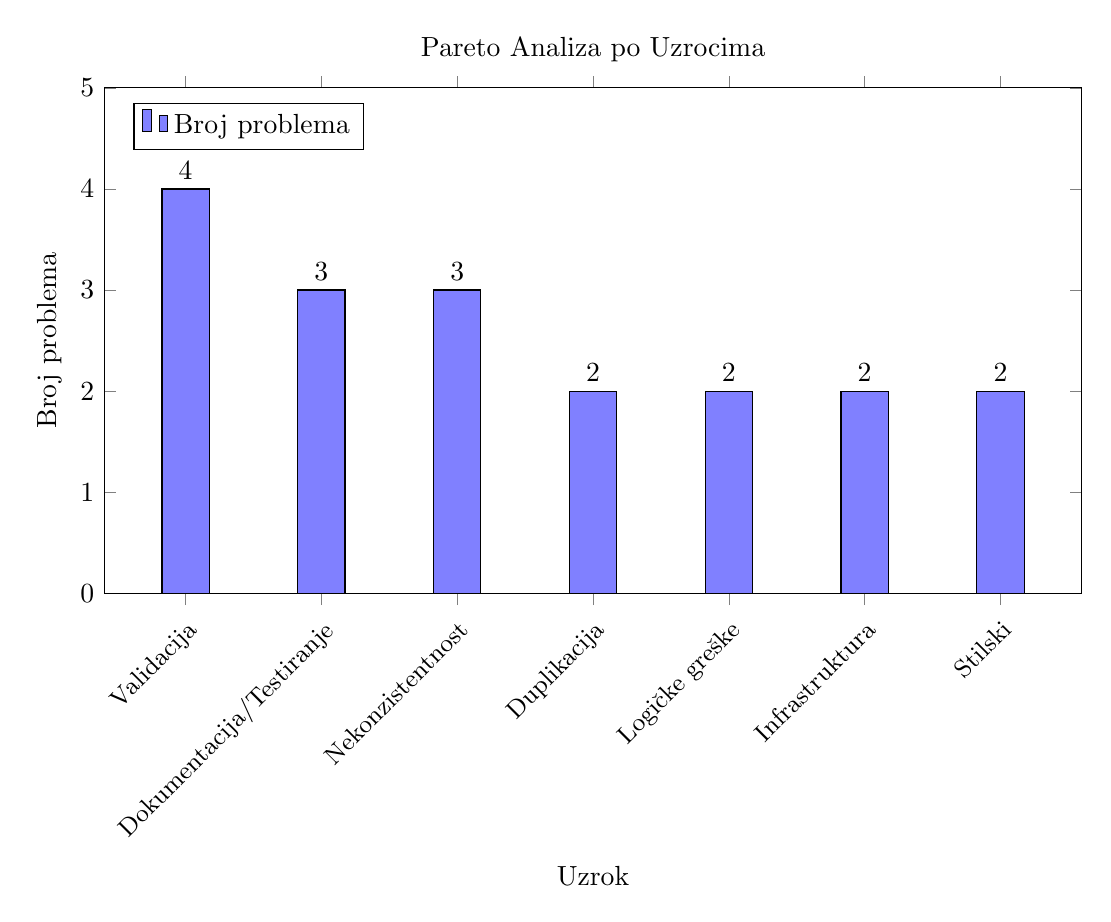
\begin{tikzpicture}
\begin{axis}[
    ybar,
    bar width=0.6cm,
    width=14cm,
    height=8cm,
    ylabel={Broj problema},
    xlabel={Uzrok},
    symbolic x coords={Validacija, Dokumentacija/Testiranje, Nekonzistentnost, Duplikacija, Logičke greške, Infrastruktura, Stilski},
    xtick=data,
    xticklabel style={rotate=45, anchor=north east, font=\small},
    ymin=0,
    ymax=5,
    legend pos=north west,
    title={Pareto Analiza po Uzrocima},
    nodes near coords,
    nodes near coords align={vertical},
]
\addplot[fill=blue!50] coordinates {
    (Validacija, 4)
    (Dokumentacija/Testiranje, 3)
    (Nekonzistentnost, 3)
    (Duplikacija, 2)
    (Logičke greške, 2)
    (Infrastruktura, 2)
    (Stilski, 2)
};
\legend{Broj problema}
\end{axis}
\end{tikzpicture}
\caption{Pareto dijagram - Analiza po uzrocima (sortirano po broju problema)}
\end{figure}

\begin{table}[H]
\centering
\begin{tabular}{lcc}
\toprule
\textbf{Uzrok} & \textbf{Broj} & \textbf{Kumulativni postotak} \\
\midrule
Validacija & 4 & 22.2\% \\
Dokumentacija/Testiranje & 3 & 38.9\% \\
Nekonzistentnost & 3 & 55.6\% \\
Duplikacija & 2 & 66.7\% \\
Logičke greške & 2 & 77.8\% \\
Infrastruktura & 2 & 88.9\% \\
Stilski & 2 & 100.0\% \\
\bottomrule
\end{tabular}
\caption{Kumulativna analiza po uzrocima}
\end{table}

\begin{figure}[H]
\centering
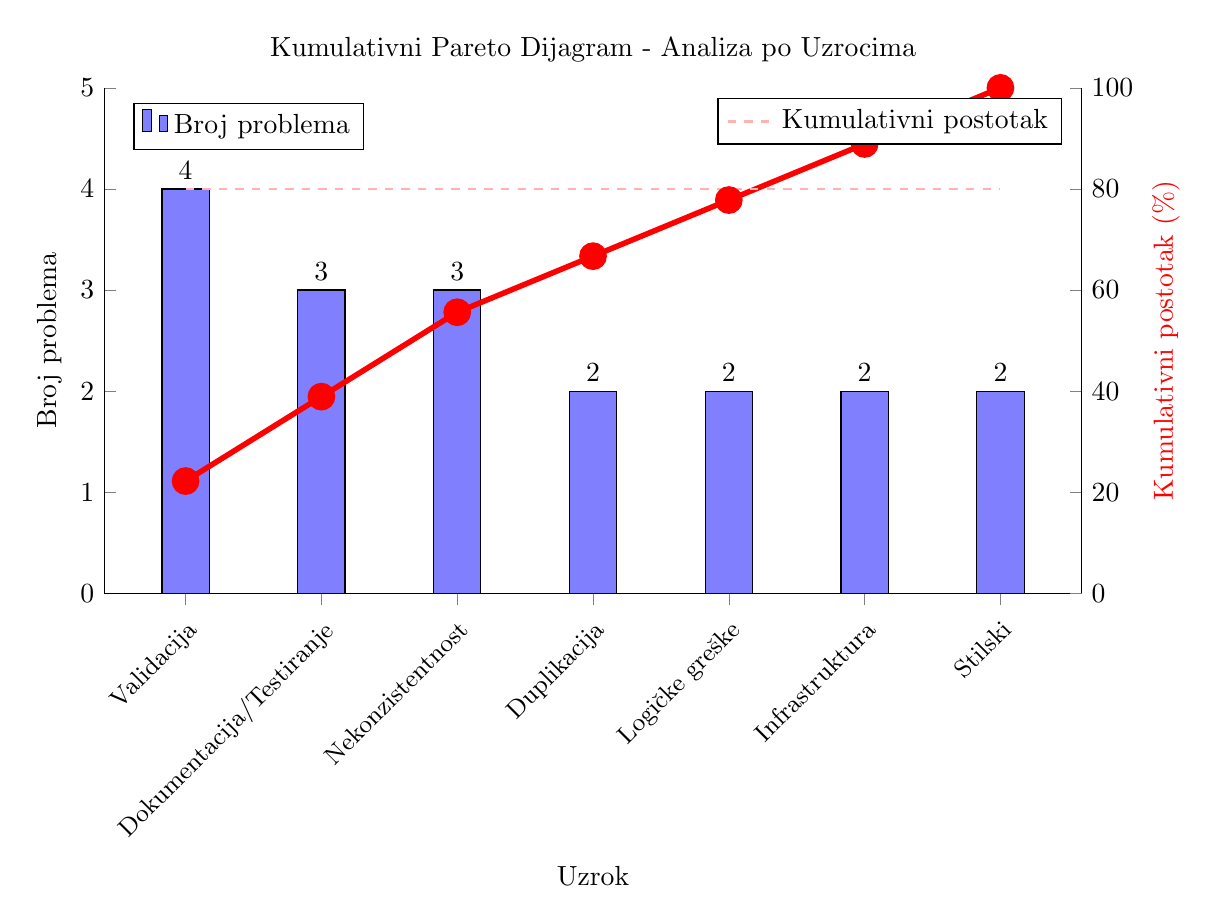
\begin{tikzpicture}
\begin{axis}[
    ybar,
    bar width=0.6cm,
    width=14cm,
    height=8cm,
    ylabel={Broj problema},
    xlabel={Uzrok},
    symbolic x coords={Validacija, Dokumentacija/Testiranje, Nekonzistentnost, Duplikacija, Logičke greške, Infrastruktura, Stilski},
    xtick=data,
    xticklabel style={rotate=45, anchor=north east, font=\small},
    ymin=0,
    ymax=5,
    legend pos=north west,
    title={Kumulativni Pareto Dijagram - Analiza po Uzrocima},
    nodes near coords,
    nodes near coords align={vertical},
    axis y line*=left,
    axis x line*=bottom,
]
\addplot[fill=blue!50] coordinates {
    (Validacija, 4)
    (Dokumentacija/Testiranje, 3)
    (Nekonzistentnost, 3)
    (Duplikacija, 2)
    (Logičke greške, 2)
    (Infrastruktura, 2)
    (Stilski, 2)
};
\legend{Broj problema}
\end{axis}
\begin{axis}[
    width=14cm,
    height=8cm,
    ylabel={Kumulativni postotak (\%)},
    ylabel style={color=red},
    ymin=0,
    ymax=100,
    axis y line*=right,
    axis x line=none,
    symbolic x coords={Validacija, Dokumentacija/Testiranje, Nekonzistentnost, Duplikacija, Logičke greške, Infrastruktura, Stilski},
    xtick=data,
    xticklabel style={rotate=45, anchor=north east, font=\small},
    legend style={at={(0.98,0.98)}, anchor=north east}
]
\addplot[color=red, mark=*, line width=2pt, mark size=4pt] coordinates {
    (Validacija, 22.2)
    (Dokumentacija/Testiranje, 38.9)
    (Nekonzistentnost, 55.6)
    (Duplikacija, 66.7)
    (Logičke greške, 77.8)
    (Infrastruktura, 88.9)
    (Stilski, 100.0)
};
\addplot[color=red!30, dashed, line width=1pt] coordinates {
    (Validacija, 80)
    (Stilski, 80)
};
\legend{, Kumulativni postotak, 80\% linija}
\end{axis}
\end{tikzpicture}
\caption{Kumulativni Pareto dijagram - Analiza po uzrocima (stapici: broj problema, linija: kumulativni postotak)}
\end{figure}

\textbf{80/20 Pravilo:}

Top 3 uzroka (Validacija, Dokumentacija/Testiranje, Nekonzistentnost) čine \textbf{55.6\%} svih problema. Top 4 uzroka čine \textbf{66.7\%} svih problema, što je blizu 80/20 principa. Fokusiranje na ove kategorije bi riješilo većinu problema.

\subsection{Pareto Analiza po Defektima}

Analizom problema po tipovima defekata i njihovoj ozbiljnosti:

\begin{table}[H]
\centering
\begin{tabular}{lccc}
\toprule
\textbf{Tip Defekta} & \textbf{Broj} & \textbf{Ozbiljnost} & \textbf{Prioritet} \\
\midrule
NullReferenceException rizici & 2 & \textcolor{critical}{Kritična} & P1 \\
FormatException rizici & 1 & \textcolor{critical}{Kritična} & P1 \\
Logičke greške & 1 & \textcolor{critical}{Kritična} & P1 \\
Duplikacija koda & 1 & \textcolor{high}{Visoka} & P2 \\
Nedostaje validacija & 4 & \textcolor{high}{Visoka} & P2 \\
Nedostaje logging & 1 & \textcolor{high}{Visoka} & P2 \\
Nedostaju testovi & 1 & \textcolor{high}{Visoka} & P2 \\
Nedostaje dokumentacija & 1 & \textcolor{high}{Visoka} & P2 \\
Arhitektonski problemi & 2 & \textcolor{medium}{Srednja} & P3 \\
Stilski problemi & 3 & \textcolor{low}{Niska} & P4 \\
\bottomrule
\end{tabular}
\caption{Analiza problema po tipovima defekata}
\end{table}

\begin{figure}[H]
\centering
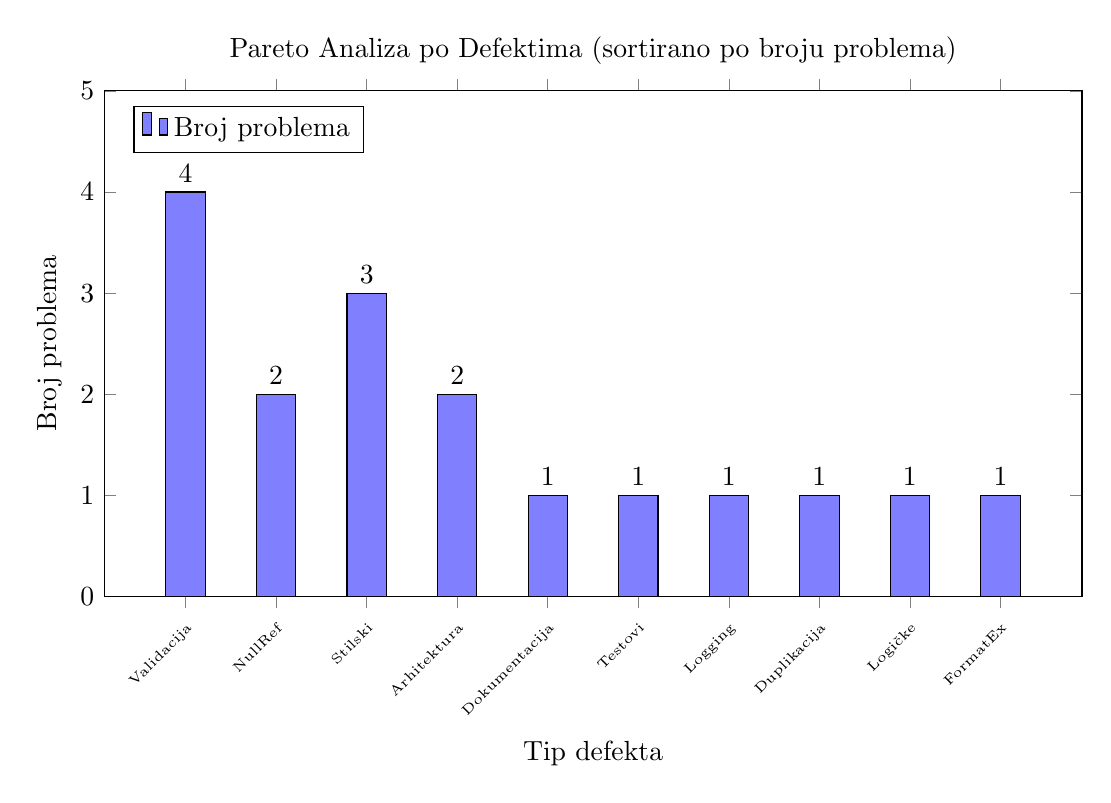
\begin{tikzpicture}
\begin{axis}[
    ybar,
    bar width=0.5cm,
    width=14cm,
    height=8cm,
    ylabel={Broj problema},
    xlabel={Tip defekta},
    symbolic x coords={Validacija, NullRef, Stilski, Arhitektura, Dokumentacija, Testovi, Logging, Duplikacija, Logičke, FormatEx},
    xtick=data,
    xticklabel style={rotate=45, anchor=north east, font=\tiny},
    ymin=0,
    ymax=5,
    legend pos=north west,
    title={Pareto Analiza po Defektima (sortirano po broju problema)},
    nodes near coords,
    nodes near coords align={vertical},
]
\addplot[fill=blue!50] coordinates {
    (Validacija, 4)
    (NullRef, 2)
    (Stilski, 3)
    (Arhitektura, 2)
    (Dokumentacija, 1)
    (Testovi, 1)
    (Logging, 1)
    (Duplikacija, 1)
    (Logičke, 1)
    (FormatEx, 1)
};
\legend{Broj problema}
\end{axis}
\end{tikzpicture}
\caption{Pareto dijagram - Analiza po defektima (sortirano po broju problema)}
\end{figure}

\begin{table}[H]
\centering
\begin{tabular}{lcc}
\toprule
\textbf{Tip Defekta} & \textbf{Broj} & \textbf{Kumulativni postotak} \\
\midrule
Validacija & 4 & 23.5\% \\
Stilski & 3 & 41.2\% \\
NullRef & 2 & 52.9\% \\
Arhitektura & 2 & 64.7\% \\
Dokumentacija & 1 & 70.6\% \\
Testovi & 1 & 76.5\% \\
Logging & 1 & 82.4\% \\
Duplikacija & 1 & 88.2\% \\
Logičke & 1 & 94.1\% \\
FormatEx & 1 & 100.0\% \\
\bottomrule
\end{tabular}
\caption{Kumulativna analiza po defektima}
\end{table}

\begin{figure}[H]
\centering
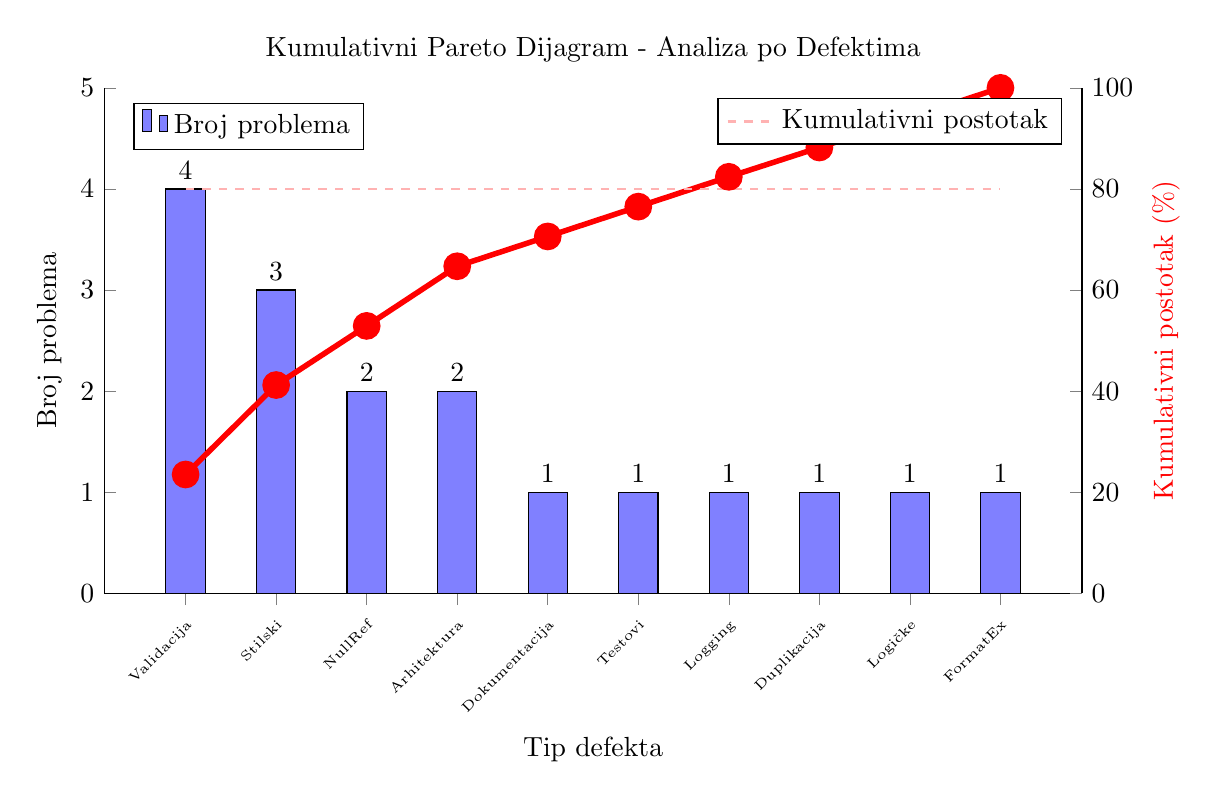
\begin{tikzpicture}
\begin{axis}[
    ybar,
    bar width=0.5cm,
    width=14cm,
    height=8cm,
    ylabel={Broj problema},
    xlabel={Tip defekta},
    symbolic x coords={Validacija, Stilski, NullRef, Arhitektura, Dokumentacija, Testovi, Logging, Duplikacija, Logičke, FormatEx},
    xtick=data,
    xticklabel style={rotate=45, anchor=north east, font=\tiny},
    ymin=0,
    ymax=5,
    legend pos=north west,
    title={Kumulativni Pareto Dijagram - Analiza po Defektima},
    nodes near coords,
    nodes near coords align={vertical},
    axis y line*=left,
    axis x line*=bottom,
]
\addplot[fill=blue!50] coordinates {
    (Validacija, 4)
    (Stilski, 3)
    (NullRef, 2)
    (Arhitektura, 2)
    (Dokumentacija, 1)
    (Testovi, 1)
    (Logging, 1)
    (Duplikacija, 1)
    (Logičke, 1)
    (FormatEx, 1)
};
\legend{Broj problema}
\end{axis}
\begin{axis}[
    width=14cm,
    height=8cm,
    ylabel={Kumulativni postotak (\%)},
    ylabel style={color=red},
    ymin=0,
    ymax=100,
    axis y line*=right,
    axis x line=none,
    symbolic x coords={Validacija, Stilski, NullRef, Arhitektura, Dokumentacija, Testovi, Logging, Duplikacija, Logičke, FormatEx},
    xtick=data,
    xticklabel style={rotate=45, anchor=north east, font=\tiny},
    legend style={at={(0.98,0.98)}, anchor=north east}
]
\addplot[color=red, mark=*, line width=2pt, mark size=4pt] coordinates {
    (Validacija, 23.5)
    (Stilski, 41.2)
    (NullRef, 52.9)
    (Arhitektura, 64.7)
    (Dokumentacija, 70.6)
    (Testovi, 76.5)
    (Logging, 82.4)
    (Duplikacija, 88.2)
    (Logičke, 94.1)
    (FormatEx, 100.0)
};
\addplot[color=red!30, dashed, line width=1pt] coordinates {
    (Validacija, 80)
    (FormatEx, 80)
};
\legend{, Kumulativni postotak, 80\% linija}
\end{axis}
\end{tikzpicture}
\caption{Kumulativni Pareto dijagram - Analiza po defektima (stapici: broj problema, linija: kumulativni postotak)}
\end{figure}

\subsection{Analiza Prioriteta}

\begin{table}[H]
\centering
\begin{tabular}{lcc}
\toprule
\textbf{Prioritet} & \textbf{Broj Problema} & \textbf{Postotak} \\
\midrule
P1 (Kritično) & 4 & 26.7\% \\
P2 (Visoko) & 8 & 53.3\% \\
P3 (Srednje) & 2 & 13.3\% \\
P4 (Nisko) & 2 & 13.3\% \\
\bottomrule
\end{tabular}
\caption{Raspodjela problema po prioritetima}
\end{table}

\textit{Napomena: Ukupno 15 problema, ali neki problemi mogu imati više prioriteta.}

\textbf{Preporuke:}
\begin{itemize}
    \item \textbf{P1 (Kritično):} 4 problema - mora se riješiti odmah prije puštanja u produkciju
    \item \textbf{P2 (Visoko):} 8 problema - riješiti u narednom sprintu
    \item \textbf{P3 (Srednje):} 2 problema - riješiti kada bude vremena
    \item \textbf{P4 (Nisko):} 2 problema - riješiti kao cleanup
\end{itemize}

\section{Dobre Prakse}

Tokom inspekcije, identifikovane su i dobre prakse u kodu:

\begin{itemize}
    \item \textbf{Separation of Concerns:} Kod je dobro organizovan u modele i servise
    \item \textbf{Enum korištenje:} Dobro korištenje enuma za \texttt{Kategorija} i sortiranje
    \item \textbf{Korištenje LINQ:} Efektivno korištenje LINQ za filtriranje i pretraživanje
    \item \textbf{Try-catch blokovi:} Postoje try-catch blokovi u \texttt{Main} metodi
    \item \textbf{CultureInfo:} Korištenje \texttt{CultureInfo.InvariantCulture} za parsiranje brojeva
    \item \textbf{StringComparison:} Korištenje \texttt{StringComparison.OrdinalIgnoreCase} za case-insensitive poređenje
\end{itemize}

\section{Preporuke za Poboljšanje}

\subsection{Kratkoročne (Sprint 1)}

\begin{enumerate}
    \item Popraviti kritične greške (ISSUE-001, ISSUE-002, ISSUE-003)
    \item Dodati validaciju inputa na svim mjestima
    \item Ukloniti duplikaciju koda (ISSUE-004)
    \item Dodati osnovni logging
\end{enumerate}

\subsection{Srednjoročne (Sprint 2-3)}

\begin{enumerate}
    \item Dodati unit testove
    \item Integrirati dependency injection
    \item Dodati konfiguracijski fajl
    \item Standardizovati imenovanje
\end{enumerate}

\subsection{Dugoročne (Sprint 4+)}

\begin{enumerate}
    \item Dodati kompletnu dokumentaciju
    \item Implementirati CI/CD pipeline
    \item Dodati integracijske testove
    \item Razmotriti migraciju na web API ili desktop aplikaciju
\end{enumerate}

\section{Komentari za Kod}

Ova sekcija sadrži detaljne komentare za kod koji su identifikovani tokom inspekcije. Komentari su organizovani po fajlovima i linijama koda, sa referencama na ISSUE-ove i checklist stavke.

\subsection{Komentari za \texttt{Program.cs}}

\subsubsection{Komentar 1: Linija 134 - ISSUE-002}

\textbf{Lokacija:} \texttt{Program.cs:134} \\
\textbf{ISSUE:} ISSUE-002 \\
\textbf{Ozbiljnost:} \textcolor{critical}{Kritična} \\
\textbf{Prioritet:} P1 (Kritično) \\
\textbf{Checklist:} CL-01 (Validacija Inputa), CL-02 (Error Handling) \\

\textbf{Kod:}
\begin{lstlisting}[language=CSharp, basicstyle=\small, numbers=left, numberstyle=\tiny, firstnumber=134]
double cijena = string.IsNullOrWhiteSpace(unos) ? 0 : double.Parse(unos, CultureInfo.InvariantCulture);
\end{lstlisting}

\textbf{Problem:} \texttt{double.Parse} može baciti \texttt{FormatException} ako korisnik unese nevalidan string (npr. "abc"). Ova greška nije uhvaćena i može dovesti do crash-a aplikacije.

\textbf{Preporuka:}
\begin{lstlisting}[language=CSharp, basicstyle=\small]
double cijena = 0;
if (!string.IsNullOrWhiteSpace(unos))
{
    if (!double.TryParse(unos, NumberStyles.Float, CultureInfo.InvariantCulture, out cijena))
    {
        Console.WriteLine("Neispravan unos cijene! Koristit će se 0.");
        cijena = 0;
    }
}
\end{lstlisting}

\subsubsection{Komentar 2: Linija 83-87 - ISSUE-005}

\textbf{Lokacija:} \texttt{Program.cs:83-87} \\
\textbf{ISSUE:} ISSUE-005 \\
\textbf{Ozbiljnost:} \textcolor{high}{Visoka} \\
\textbf{Prioritet:} P2 (Visoko) \\
\textbf{Checklist:} CL-01 (Validacija Inputa) \\

\textbf{Kod:}
\begin{lstlisting}[language=CSharp, basicstyle=\small, numbers=left, numberstyle=\tiny, firstnumber=83]
Console.Write("Naziv: ");
string naziv = Console.ReadLine();

Console.Write("Opis: ");
string opis = Console.ReadLine();
\end{lstlisting}

\textbf{Problem:} Nema validacije da li su \texttt{naziv} i \texttt{opis} prazni. Ako korisnik unese prazan string, stavka će biti kreirana sa praznim nazivom, što može dovesti do problema.

\textbf{Preporuka:}
\begin{lstlisting}[language=CSharp, basicstyle=\small]
string naziv;
do
{
    Console.Write("Naziv: ");
    naziv = Console.ReadLine();
    if (string.IsNullOrWhiteSpace(naziv))
        Console.WriteLine("Naziv ne može biti prazan!");
} while (string.IsNullOrWhiteSpace(naziv));
\end{lstlisting}

\subsubsection{Komentar 3: Linija 221-224 - ISSUE-005, ISSUE-013}

\textbf{Lokacija:} \texttt{Program.cs:221-224} \\
\textbf{ISSUE:} ISSUE-005, ISSUE-013 \\
\textbf{Ozbiljnost:} \textcolor{high}{Visoka}, \textcolor{medium}{Srednja} \\
\textbf{Prioritet:} P2 (Visoko), P3 (Srednje) \\
\textbf{Checklist:} CL-01 (Validacija Inputa), CL-17 (User Experience) \\

\textbf{Kod:}
\begin{lstlisting}[language=CSharp, basicstyle=\small, numbers=left, numberstyle=\tiny, firstnumber=221]
Console.Write("Unesi naziv stavke za uklanjanje: ");
string naziv = Console.ReadLine();
inventarService.UkloniStavku(naziv);
Console.WriteLine("Ako je stavka postojala, uklonjena je.");
\end{lstlisting}

\textbf{Problem:}
\begin{enumerate}
    \item Nema provjere da li je \texttt{naziv} prazan
    \item Poruka "Ako je stavka postojala, uklonjena je." je loša UX - korisnik ne zna da li je stavka stvarno uklonjena
\end{enumerate}

\textbf{Preporuka:}
\begin{lstlisting}[language=CSharp, basicstyle=\small]
Console.Write("Unesi naziv stavke za uklanjanje: ");
string naziv = Console.ReadLine();
if (string.IsNullOrWhiteSpace(naziv))
{
    Console.WriteLine("Naziv ne može biti prazan!");
    return;
}

var stavka = inventarService.Pretrazi(new Filter(naziv: naziv)).FirstOrDefault();
if (stavka == null)
{
    Console.WriteLine($"Stavka '{naziv}' nije pronađena.");
    return;
}

inventarService.UkloniStavku(naziv);
Console.WriteLine($"Stavka '{naziv}' je uspješno uklonjena.");
\end{lstlisting}

\subsubsection{Komentar 4: Linija 236 - ISSUE-013}

\textbf{Lokacija:} \texttt{Program.cs:236} \\
\textbf{ISSUE:} ISSUE-013 \\
\textbf{Ozbiljnost:} \textcolor{medium}{Srednja} \\
\textbf{Prioritet:} P3 (Srednje) \\
\textbf{Checklist:} CL-16 (Edge Cases) \\

\textbf{Kod:}
\begin{lstlisting}[language=CSharp, basicstyle=\small, numbers=left, numberstyle=\tiny, firstnumber=236]
var stavka = inventarService.Pretrazi(new Filter(naziv: naziv)).FirstOrDefault();
\end{lstlisting}

\textbf{Problem:} Ako postoji više stavki sa istim nazivom, uzima se samo prva. To može biti neočekivano ponašanje.

\textbf{Preporuka:}
\begin{lstlisting}[language=CSharp, basicstyle=\small]
var stavke = inventarService.Pretrazi(new Filter(naziv: naziv)).ToList();
if (stavke.Count == 0)
{
    Console.WriteLine($"Stavka '{naziv}' nije pronađena.");
    return;
}
if (stavke.Count > 1)
{
    Console.WriteLine($"Upozorenje: Pronađeno je {stavke.Count} stavki sa nazivom '{naziv}'. Ažuriraće se prva.");
}
var stavka = stavke.First();
\end{lstlisting}

\subsubsection{Komentar 5: Linija 288-294 - ISSUE-013}

\textbf{Lokacija:} \texttt{Program.cs:288-294} \\
\textbf{ISSUE:} ISSUE-013 \\
\textbf{Ozbiljnost:} \textcolor{medium}{Srednja} \\
\textbf{Prioritet:} P3 (Srednje) \\
\textbf{Checklist:} CL-01 (Validacija Inputa), CL-16 (Edge Cases) \\

\textbf{Kod:}
\begin{lstlisting}[language=CSharp, basicstyle=\small, numbers=left, numberstyle=\tiny, firstnumber=288]
Console.Write("Unesi početni datum (yyyy-MM-dd) ili prazno: ");
if (DateTime.TryParse(Console.ReadLine(), out DateTime dtPocetak))
    izvjestaj.PocetakPerioda = dtPocetak;

Console.Write("Unesi krajnji datum (yyyy-MM-dd) ili prazno: ");
if (DateTime.TryParse(Console.ReadLine(), out DateTime dtKraj))
    izvjestaj.KrajPerioda = dtKraj;
\end{lstlisting}

\textbf{Problem:} Nema provjere da li je početni datum prije krajnjeg datuma. Ako korisnik unese neispravan raspon datuma, aplikacija će nastaviti sa generisanjem izvještaja sa neispravnim podacima.

\textbf{Preporuka:}
\begin{lstlisting}[language=CSharp, basicstyle=\small]
if (izvjestaj.PocetakPerioda.HasValue && izvjestaj.KrajPerioda.HasValue &&
    izvjestaj.PocetakPerioda.Value > izvjestaj.KrajPerioda.Value)
{
    Console.WriteLine("Greška: Početni datum mora biti prije krajnjeg datuma!");
    return;
}
\end{lstlisting}

\subsection{Komentari za \texttt{Services/InventarService.cs}}

\subsubsection{Komentar 6: Linija 22-24 - ISSUE-001}

\textbf{Lokacija:} \texttt{Services/InventarService.cs:22-24} \\
\textbf{ISSUE:} ISSUE-001 \\
\textbf{Ozbiljnost:} \textcolor{critical}{Kritična} \\
\textbf{Prioritet:} P1 (Kritično) \\
\textbf{Checklist:} CL-01 (Validacija Inputa), CL-03 (Null Safety) \\

\textbf{Kod:}
\begin{lstlisting}[language=CSharp, basicstyle=\small, numbers=left, numberstyle=\tiny, firstnumber=22]
if (inventar.Stavke.Any(s => s.Naziv.Equals(stavka.Naziv, StringComparison.OrdinalIgnoreCase) &&
                             s.Dobavljac.Equals(stavka.Dobavljac, StringComparison.OrdinalIgnoreCase)))
\end{lstlisting}

\textbf{Problem:} Ako \texttt{stavka.Dobavljac} ili postojeća stavka u listi ima \texttt{null} vrijednost za \texttt{Dobavljac}, poziv \texttt{Equals} će baciti \texttt{NullReferenceException}.

\textbf{Preporuka:}
\begin{lstlisting}[language=CSharp, basicstyle=\small]
if (inventar.Stavke.Any(s =>
    string.Equals(s.Naziv, stavka.Naziv, StringComparison.OrdinalIgnoreCase) &&
    string.Equals(s.Dobavljac ?? "", stavka.Dobavljac ?? "", StringComparison.OrdinalIgnoreCase)))
\end{lstlisting}

\subsubsection{Komentar 7: Linija 47-82 - ISSUE-004}

\textbf{Lokacija:} \texttt{Services/InventarService.cs:47-82} \\
\textbf{ISSUE:} ISSUE-004 \\
\textbf{Ozbiljnost:} \textcolor{high}{Visoka} \\
\textbf{Prioritet:} P2 (Visoko) \\
\textbf{Checklist:} CL-05 (DRY Princip) \\

\textbf{Problem:} Metoda \texttt{Pretrazi} ima identičnu logiku kao \texttt{FilterService.PrimijeniFilter}. Ovo je duplikacija koda koja otežava održavanje.

\textbf{Preporuka:} Refaktorisati da koristi \texttt{FilterService}:
\begin{lstlisting}[language=CSharp, basicstyle=\small]
public List<StavkaInventara> Pretrazi(Filter filter)
{
    if (filter == null) throw new ArgumentNullException(nameof(filter));
    return FilterService.PrimijeniFilter(inventar.Stavke, filter);
}
\end{lstlisting}

\subsection{Komentari za \texttt{Services/StavkaInventaraService.cs}}

\subsubsection{Komentar 8: Linija 8-24 - ISSUE-003}

\textbf{Lokacija:} \texttt{Services/StavkaInventaraService.cs:8-24} \\
\textbf{ISSUE:} ISSUE-003 \\
\textbf{Ozbiljnost:} \textcolor{critical}{Kritična} \\
\textbf{Prioritet:} P1 (Kritično) \\
\textbf{Checklist:} CL-04 (Logika Aplikacije) \\

\textbf{Kod:}
\begin{lstlisting}[language=CSharp, basicstyle=\small, numbers=left, numberstyle=\tiny, firstnumber=8]
public static bool JeKriticna(StavkaInventara stavka)
{
    if (stavka.Kolicina < stavka.MinKolicina)
    {
        if (stavka.DatumNabavke < DateTime.Now.AddDays(-30))
            return true;

        if (stavka.Kategorija == Kategorija.Hrana || stavka.Kategorija == Kategorija.Pice)
            return true;

        return true; // Ova linija je uvijek dostupna
    }
    // ...
}
\end{lstlisting}

\textbf{Problem:} Metoda \texttt{JeKriticna} ima logičku grešku. Ako je \texttt{stavka.Kolicina < stavka.MinKolicina}, metoda uvijek vraća \texttt{true} bez obzira na ostale uslove. Linija 18 (\texttt{return true;}) je unreachable code jer se uvijek izvršava.

\textbf{Preporuka:} Refaktorisati logiku:
\begin{lstlisting}[language=CSharp, basicstyle=\small]
public static bool JeKriticna(StavkaInventara stavka)
{
    if (stavka == null) return false;

    const int KRITICNI_PERIOD_DANA = 30;
    const int MAKSIMALNI_PERIOD_DANA = 60;

    // Kritično ako je količina ispod minimuma
    bool ispodMinimuma = stavka.Kolicina < stavka.MinKolicina;

    // Posebno kritično za hranu i piće
    bool hranaIliPice = stavka.Kategorija == Kategorija.Hrana ||
                        stavka.Kategorija == Kategorija.Pice;

    // Kritično ako je stara
    bool stara = (DateTime.Now - stavka.DatumNabavke).TotalDays > MAKSIMALNI_PERIOD_DANA;
    bool staraIKriticna = stavka.DatumNabavke < DateTime.Now.AddDays(-KRITICNI_PERIOD_DANA);

    return ispodMinimuma && (hranaIliPice || staraIKriticna) || stara;
}
\end{lstlisting}

\subsubsection{Komentar 9: Linija 12, 21 - ISSUE-010}

\textbf{Lokacija:} \texttt{Services/StavkaInventaraService.cs:12, 21} \\
\textbf{ISSUE:} ISSUE-010 \\
\textbf{Ozbiljnost:} \textcolor{high}{Visoka} \\
\textbf{Prioritet:} P2 (Visoko) \\
\textbf{Checklist:} CL-07 (Konfiguracija) \\

\textbf{Kod:}
\begin{lstlisting}[language=CSharp, basicstyle=\small, numbers=left, numberstyle=\tiny, firstnumber=12]
if (stavka.DatumNabavke < DateTime.Now.AddDays(-30))  // Magic number
\end{lstlisting}
\begin{lstlisting}[language=CSharp, basicstyle=\small, numbers=left, numberstyle=\tiny, firstnumber=21]
if ((DateTime.Now - stavka.DatumNabavke).TotalDays > 60)  // Magic number
\end{lstlisting}

\textbf{Problem:} Hardcoded vrijednosti 30 i 60 dana su "magic numbers" koje otežavaju održavanje.

\textbf{Preporuka:} Premjestiti u konstante ili konfiguraciju:
\begin{lstlisting}[language=CSharp, basicstyle=\small]
private const int KRITICNI_PERIOD_DANA = 30;
private const int MAKSIMALNI_PERIOD_DANA = 60;
\end{lstlisting}

\subsection{Komentari za \texttt{Services/FilterService.cs}}

\subsubsection{Komentar 10: Cijeli fajl - ISSUE-004, ISSUE-015}

\textbf{Lokacija:} \texttt{Services/FilterService.cs} \\
\textbf{ISSUE:} ISSUE-004, ISSUE-015 \\
\textbf{Ozbiljnost:} \textcolor{high}{Visoka}, \textcolor{low}{Niska} \\
\textbf{Prioritet:} P2 (Visoko), P4 (Nisko) \\
\textbf{Checklist:} CL-05 (DRY Princip), CL-06 (Održivost Koda) \\

\textbf{Problem:} \texttt{FilterService} postoji ali se ne koristi nigdje u aplikaciji. Ista logika je implementirana u \texttt{InventarService.Pretrazi}.

\textbf{Preporuka:}
\begin{itemize}
    \item Ili koristiti \texttt{FilterService} u \texttt{InventarService.Pretrazi} (preporučeno)
    \item Ili ukloniti \texttt{FilterService} ako se ne planira koristiti
\end{itemize}

\section{Checklist za Pull Request}

\begin{itemize}
    \item[$\square$] Svi P1 problemi su riješeni
    \item[$\square$] Dodana je validacija na svim mjestima gdje se prima input
    \item[$\square$] Uklonjena je duplikacija koda
    \item[$\square$] Dodani su osnovni unit testovi
    \item[$\square$] Dodana je osnovna dokumentacija (README.md)
    \item[$\square$] Kod je prošao code review
    \item[$\square$] Nema compiler warnings
    \item[$\square$] Kod je formatiran prema standardima
\end{itemize}

\section{Zaključak}

Aplikacija \textbf{RestaurantInventory} ima dobru osnovnu strukturu i separation of concerns, ali ima nekoliko kritičnih problema koji moraju biti riješeni prije produkcije. 

\textbf{Najveći problemi su:}
\begin{enumerate}
    \item \textbf{Kritične greške} koje mogu dovesti do crash-a aplikacije (NullReferenceException, FormatException, logičke greške)
    \item \textbf{Nedostaje validacija} na više mjesta što može dovesti do neočekivanog ponašanja
    \item \textbf{Nedostaju testovi i dokumentacija} što otežava održavanje i razvoj
\end{enumerate}

\textbf{Pareto analiza} pokazuje da se fokusiranjem na tri glavna uzroka (Validacija, Dokumentacija/Testiranje, Nekonzistentnost) može riješiti 66.7\% svih problema.

\textbf{Preporučeno je riješiti sve P1 i P2 probleme prije puštanja u produkciju.}

\vspace{2cm}

\begin{center}
\rule{0.5\textwidth}{0.4pt}

\textbf{Kreirao:} Bakir Činjarević \\
\textbf{Datum:} \today \\
\textbf{Verzija izvještaja:} 1.0
\end{center}

\end{document}

